\begin{figure}[!tp]
	\centering
	\begin{minipage}[!t]{\textwidth}
		\centering
		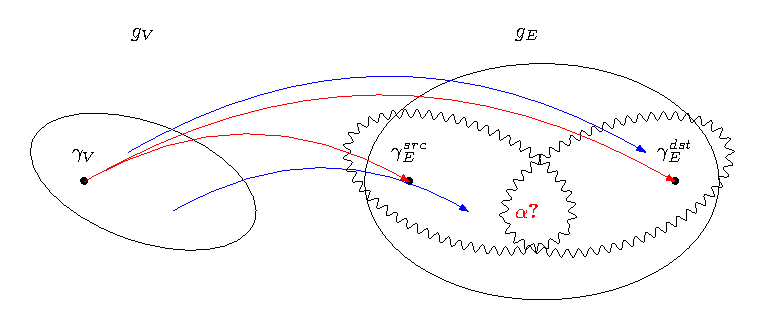
\includegraphics[width=\textwidth]{images/nesting/patterns/01_preliminar_question.pdf}
		\subcaption{Comparing the vertex summarization pattern and the path summarization patterns. We suppose that edge grouping references ($\gamma_E^{src}$ and $\gamma_E^{dst}$) correspond to the same vertex appearing as a vertex grouping reference ($\gamma_V$) Such correspondence is directly marked my the user itself providing the query by drawing morphisms (correspondences) between the vertex and the path summarization patterns (red edges). The intersections between the two patterns may be directly outlined by the user itself that provides the query (blue edges, representing other morphisms).}
		\label{fig:patcomparison}
	\end{minipage} \begin{minipage}[!t]{0.45\textwidth}
		\centering
		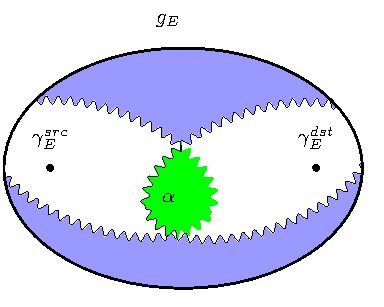
\includegraphics[width=1\textwidth]{images/nesting/patterns/02_edge_analysis.pdf}
		\subcaption{Path summarization pattern sharing an $\alpha$ area of common patterns shared between the patterns, which are necessairly not the edge grouping references by definition.}
		\label{fig:edgewithIntersectionNonSRC}
	\end{minipage}\quad \begin{minipage}[!t]{0.45\textwidth}
		\centering
		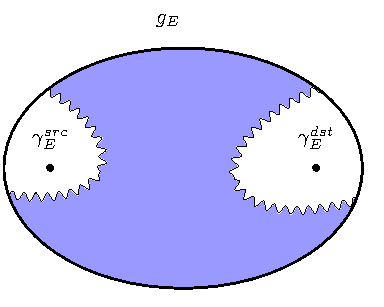
\includegraphics[width=1\textwidth]{images/nesting/patterns/03_edge_analysis.pdf}
		\subcaption{Path summarization pattern not sharing a common $\alpha$ area, although $\gamma_E^{src}$ and $\gamma_E^{dst}$ must always be present in $g_E$ by hypothesis. This constraint guarantees that the newly created edge will be associated to a nested vertex originating from the vertex summarization pattern.}
		\label{fig:edgeWithNoIntersection}
	\end{minipage}
	\caption{Vertex (V) and Path (E) summarization patterns for the query expressed in Example \vref{ex:nestingbib}. Vertex and edge grouping references are marked by a light blue circled node. As we can see, the vertex grouping reference depicts the same property expressed by edge grouping references.}
	\label{fig:patternAnalysis}
\end{figure}
\section{Class of optimizable graph nesting queries}\label{sec:optimizableClass}
Prior to the analysis of the THoSP algorithm that is going to be provided later on in the next subsection, we want to discuss which is the class of vertex and path summarization patterns optimizable as discussed in the chapter's introduction. As we already observed, %, the comparison of several graph collections may lead to an intractable solution which is exponential in time over the graph dimension, where the exponent is the arbitrary size of the collection generated from the original graph operand. 
the exhaustive search of graph patterns in the most general scenario must be done at any rate, because the vertex and  edge subgraphs may be extracted by an external tool of which we totally ignore its behaviour. As we also discussed in the introduction, the generation of the collections is only relevant with respect to actual data that is going to be nested and, in our case, we can only nest a subgraph of the graph resulting from the graph visiting process: consequently, within each pattern we must remark which elements are going to be nested at the final result.

First, we must provide a formal characterization of the grouping reference: we want to elect a subgraph $\gamma_p$ for each graph pattern $g_p$ such that each graph generated by the morphisms\footnote{See Definition \vref{sec:graphamatch} for a back reference.} $m_{g_p}(\nested)$ expose unique elements referring to $\gamma_p$. %each for each nested graph $\nested$, a \textit{grouping reference} $\gamma_p$ of a graph pattern $g_p$ elects which elements of the subgraph $g\subseteq \nested$ returned by the graphs extraction query must appear only once per returned subgraph by $m_{g_p}(\nested)$. 
These grouping references allow to elect the subcomponents that identify an entity over which the aggregation will be performed during the graph matching process. Hereby, we can provide the following formal definition for grouping references:
\begin{definition}[Grouping reference]
Given a graph pattern $g_p$ generating a set of morphisms $m_{g_p}(\nested)$ over a nested graph $\nested$, a \textbf{grouping reference} $\gamma_p$ is a subpattern $\gamma_p\subseteq g_p$ restricting the possible morphisms generated by $m_{g_p}(\nested)$ to the $f_i$ such that $|f_i(o)|=1$ for each object $o\in O_{\gamma_p}$ and that another morphism $f_j\neq f_i$ is such that $f_i(O_{\gamma_p})\neq f_j(O_{\gamma_p})$.
\end{definition}

In particular, the elements appearing in SQL's \texttt{Group By}, AQL's \texttt{COLLECT} and Cypher's \texttt{WITH} (except from the parts where the aggregation is performed) are the grouping references of our matched graphs.

In order to reduce the computational complexity of aggregating the grouping reference, we can reduce the grouping references to one single vertex for vertex summarization patterns, and to two (distinct) vertices for path summarization patterns: in the first scenario, such vertex will identify the entity over which we can perform the nesting of all the other matched contents, while for the path summarization pattern the grouping references will identify the source ($\gamma_E^{src}$) and target ($\gamma_E^{dst}$) vertices corresponding to the vertex summarization patterns' grouping references, and hereby corresponding to the final vertices that are going to be nested in the final result. Hereby, the class of our algorithms create new nested edges only over vertices that have been previously matched as grouping references and then nested. Moreover, we can choose to mark with a specific $\xi$ value (e.g. \mstr{toNest}) each vertex and edge within each pattern in order to remark which matched vertices and edges are going to be represented in the final nesting result; this implies that UDF functions are not required by such class of problems because they can be directly represented within the graph patterns.


%\hl{Research purposes, currently investigated with the research group at Leipzig University}
%\textbf{Generalization of pattern matching approaches (algorithmical enhancement)}. Current graph query languages perform matches of different $G_H$ separately, while it can be beneficial to visit all the common subpatterns only once, and not $k$ times, thus reducing the visiting complexity from $|g|^k$ to $|g|$, where $|g|$ is the common subgraph. The application of chained generalized graph grammar rules must be done efficiently without repeating some visiting tasks more than once. The target is to find the subgraphs commonly shared by several matching strategies, whenever is possible (e.g. graph nesting as introduced in the previous chapter.)
%\textbf{Overcoming to Cypher limitations}. This algorithmical assumption implies that we do not need to extend Cypher to support nestings for some simple graph pattern matching tasks. 

Figure \vref{fig:patternAnalysis} provides an example on how  graph nesting queries based on grouping references can be optimized,for both vertex ($g_V$) and path ($g_E$) summarization queries: given that the users are going to provide both the vertex and the path summarization queries, such users must directly draw the correspondences between vertex and edge pattern queries, so that the correspondences can be promptly be identified by the query plan which can better optimize the whole query execution (\subref{fig:patcomparison}). After doing so, we can start to perform the general graph visiting algorithm for graph nesting (Algorithm \ref{alg:general}) by detecting which regions of both patterns are shared together in $\alpha=g_V\cap g_E$ (Figure \ref{fig:edgewithIntersectionNonSRC}); given that source and destination vertices in path summarization patterns' grouping references are distinct by definition, source and destination vertices may not be represented in $\alpha$ (line \ref{obtainAlpha}). Consequently, in order to reduce the graph visiting process, we can first perform pattern matching over the input graph over $\alpha$, thus allowing a partial instantiation of the $g_V$ and $g_E$ patterns, and then iteratively extend the nesting information after each visit of $\alpha$ and  its own refinements. In particular, we can perform the algorithm  as follows:
\begin{algorithm}[!t]
	\caption{Grouping Reference Optimizable Queries (GROQ)}\label{alg:general}
	\begin{adjustbox}{max width=\textwidth}
		\begin{minipage}{1.2\linewidth}
			\begin{algorithmic}[1]
				\State {\textbf{new} $\nested' := (\ngraph_{c+1}, O,\ell,\xi,\phi)$}
				\State
				\Procedure{GROQ}{$(g_V,\gamma_V),({g_E},\gamma_E^{src},\gamma_E^{dst}),m;\;\nested$}:\Comment{$\nested=(\ngraph_c,O,\ell,\xi,\phi)$}
				\State {$\alpha:=g_V\cap {g_E}\backslash(\gamma_V\cup\gamma_E)$;}\label{obtainAlpha}
				\State {lV $:=$ [];}
				\If{$\alpha\neq\emptyset$}
					\For {\textbf{each graph} $g^i$ generated from $m_\alpha(\nested)$ }\label{eachAlpha}
						\State {lV $:=\{f_i\in m_{g_V;\gamma_V}(\nested)|f_i(\alpha)=g^i\}$}
						\State {GROQ$\alpha$}{($(g_V,\gamma_V),({g_E},\gamma_E^{src},\gamma_E^{dst}),m;\;\textup{lV},\nested$)}
					\EndFor
				\Else
					\State {lV $:=m_{g_V;\gamma_V}(\nested)$}\label{complete}
					\State {GROQ$\alpha$}{($(g_V,\gamma_V),({g_E},\gamma_E^{src},\gamma_E^{dst}),m;\;\textup{lV},\nested$)}
				\EndIf
				
				\EndProcedure
				\State
				\Procedure{GROQ$\alpha$}{$(g_V,\gamma_V),({g_E},\gamma_E^{src},\gamma_E^{dst}),m;\;\textup{lV},\nested$}
				\For {\textbf{each morphism} $f_i\in\; $lV}
				\State {$\{{i}_c\}:=f_i(\gamma_V)$}\label{vertexReferencePatt}
				\State {$\ell(i_{c+1}):=\ell(i_c);\; \xi(i_{c+1}):=\xi(i_c);\; \phi(i_{c+1})=\phi(i_{c+1})|_{\dom(\phi(i_{c+1}))\backslash\{\ONTA,\RELA\}}$}\label{vertexLVPreserve}
				\State {$\phi(\ngraph_{c+1},\ONTA):=\phi(\ngraph_{c+1},\ONTA)\cup \{{i}_{c+1}\}$}\label{vertexGeneration}
				\State {$\phi({i}_{c+1},\ONTA):=\phi({i}_{c+1},\ONTA)\cup\Set{f_i(o)|o\in O_{g_V},\mstr{toNest}\in\xi(o)\wedge o\in \phi(o_{g_V},\ONTA)}$}\label{vertexContent1}
				\State {$\phi({i}_{c+1},\RELA):=\phi({i}_{c+1},\RELA)\cup\Set{f_i(o)|o\in O_{g_V},\mstr{toNest}\in\xi(o)\wedge o\in \phi(o_{g_V},\RELA)}$}\label{vertexContent2}
				\EndFor
				\For {\textbf{each morphism} $f_i,f_j\in\; $lV}
				\State{lE $:=\{f_k\in m_{{g_E};\gamma_E^{src},\gamma_E^{dst}}(\nested)|f_i(\gamma_V)=f_k(\gamma_E^{src}),f_j(\gamma_V)=f_k(\gamma_E^{dst})\}$}\label{fulTraverse}
				\For {\textbf{each morphism} $f_k\in\; $lE}
				\State {$\{s_c\}:=f_i(\gamma_E^{src})$;\qquad $\{d_c\}:=f_i(\gamma_E^{dst})$}\label{pathReferencePatt1}
				\State {$\omega:=dt(s,d)$}\label{pathReferencePatt2}
				\State {$\ell(\omega_{c+1}):=\ell(s_c)\cup\ell(d_c);\; \xi(i_{c+1}):=\xi(i_c)\cup\ell(d_c)$}\label{fromNewElements}
				\State {$\phi(\omega_{c+1},\RELA):=\phi(\omega_{c+1},\RELA)\cup f_k(\gamma_V)$}\label{edgeGeneration}
				\State {$\phi(\omega_{c+1},\SRC):=\{s_{c+1}\}$;\qquad $\phi(\omega_{c+1},\DST):=\{d_{c+1}\}$}
				\State {$\phi(\omega_{c+1},\ONTA):=\phi(\omega_{c+1},\ONTA)\cup\Set{f_k(o)|o\in O_{g_E},\mstr{toNest}\in\xi(o)\wedge o\in \phi(o_{g_E},\ONTA)}$}
				\State {$\phi(\omega_{c+1},\RELA):=\phi(\omega_{c+1},\RELA)\cup\Set{f_k(o)|o\in O_{g_E},\mstr{toNest}\in\xi(o)\wedge o\in \phi(o_{g_E},\RELA)}$}
				\EndFor
				\EndFor
				\EndProcedure
				
			\end{algorithmic}
	\end{minipage}
	\end{adjustbox}
\end{algorithm}

\begin{itemize}
\item Given a graphs extraction language $m$ (not necessarily) supporting grouping references, we extract all the subgraphs $g^i$ of $\nested$ generated by morphisms $m_\alpha(\nested)$, when $\alpha$ is not empty (line \ref{eachAlpha}). If $\alpha$ is otherwise an empty pattern, we must necessarily perform a complete visit of the vertex patterns $g_V$, and perform complete instantiations of such patterns (line \ref{complete}). 
\item Given that the nested graph representation relies on the GSM model, we can iteratively construct the nested graph without knowing the complete information by relying on the ids of the expected elements, and we can provide the greatest subgraph of $g$ matching $\alpha$  after visiting  each possible $\alpha$ matching result, represented as a morphism $f_i$. For this reason, the GROQ$\alpha$ subroutine may be called in both cases.

\item After providing a partial instantiation of the vertex summarization patterns via $\alpha$, we find a vertex $i_c$ matching the grouping reference $\gamma_V$ to which we are going to nest the remaining objects: from $i_c$ we generate a newly derived vertex $i_{c+1}$ %start to generate a new nested vertex: this new vertex $i_{c+1}$ descends from the object $i_c$ matched by the grouping reference $\gamma_V$ 
 (line \ref{vertexReferencePatt}) preserving all the labels, expressions and containments of $i_c$ (except from \RELA and \ONTA -- line \ref{vertexLVPreserve}). In particular, the nesting content of $i_{c+1}$ derives from the partial instantiation of the morphism $f_i$, by choosing the vertices and edges in $\nested$ which corresponds to vertex summarization objects marked with \mstr{toNest} (lines \ref{vertexContent1} and \ref{vertexContent2}).

\item At this point we can use the same semi-instantiated morphisms in \texttt{lV} from $\alpha$ to partially instantiate the path summarization pattern, that  is now going to be fully traversed (line \ref{fulTraverse}). For each of these $f_i$ instantiations, new edges are going to be generated, inheriting the labels, values and containments (except from \RELA and \ONTA) from the matched edges grouping references, $s_c$ and $d_c$. In particular, we can directly create associate to such edge the soruces and the targets represented by nested vertices, which will respectively be $s_{c+1}$ and $d_{c+1}$.

\item The procedure is iterated until the whole graph is not visited via subsequent morphisms, and hence all the matched elements are associated from the objects $i_{c+1}$ (either vertices or edges) generated from the ones matched by the grouping reference $i_c$.
\end{itemize}

As we can see from the algorithm, the advantage of this approach is that the graph $g^i$ and the instantiated morphisms (as a consequence of the graph matching phase) are promptly used to define the nested information (e.g., lines \ref{vertexGeneration}-\ref{vertexContent2}). It is evident that the aforementioned algorithm provides the best performances when $\gamma_E^{src}$ and $\gamma_E^{dst}$ are separated by  one edge distance in $\alpha$   and both $g_V$ and $g_E$ create graph collections that are partitions of $\nested$. On the other hand, this class of algorithms was already discussed in literature and, consequently, an approach describing how to optimize such  scenarios can be already found in literature \cite{JunghannsPR17}. Nevertheless, this chapter focuses on another types of algorithms, which are the ones where $\alpha$ contains two edges and one vertex; this class of problems, to the best of our knowledge, has not been discussed yet in current literature with respect to their optimizations. %Therefore, the next paragraph is going to introduce one specific algorithm for $\alpha\neq\emptyset$, where in particular $\alpha$ is formed by one single vertex.
 Please note that, when $\alpha=\emptyset$, the computational complexity of the algorithm may easily become quadratic ($|\phi(\ngraph,\ONTA)|+|\phi(\ngraph,\ONTA)|^2$).

\subsection{Two HOp Separated Patterns Algorithm}\label{sec:THOSPA}
We now want to focus on a specific instance of the problem stated in Algorithm \ref{alg:general}: suppose to store a graph using adjacency lists similarly to the one proposed in the Graph Join algorithm chapter (Section \vref{sec:algo}); in particular, the previous data structure is now extended with both vertex and edge containment, plus with both ingoing and outgoing edges for each single graph vertex. The latter requirement is added in order to satisfy the possibility to visit the edges backwards, thus allowing to navigate the graph in each possible direction. The main data structure over which this algorithm relies  is presented in Figure \vref{nestedGraphVertex}: it shows that minor changes have been applied to the original data structure that was used to serialize graph within the graph join scenario. %Moreover, in this case we mark with different hash values the vertices within the data structure satisfying different predicates within the predicates. 
Given that the data structure requires a simple linear visit of the graph, no additional primary and secondary data structures are required. Nevertheless, during our serialization phase we provide both a primary index for accessing external informations (\textit{VertexIndex}) and the serialization of all the vertices' adjacency lists, which is going to be used for traversing the graph (\textit{VertexVals}). In our straightforward implementation, hash values are here used only as placeholders for the nodes' labels used within the patterns but, given that vertices are not sorted by hash value as for graph joins, we keep the hash fields for both backward compatibility and in order to make graph joins possible for nested graphs, too.


Let us now restrict $\alpha$ to one single vertex and two edges: for each vertex $p_i$ matched by $\alpha$ we know that we must (possibly) visit all the edges going from $p_i$ towards the vertices $\gamma_E^{src}$ and $\gamma_E^{dst}$, that substantially are $\gamma_V$. Please note that if in $g_E$ there is no path connecting $\alpha$ to $\gamma_E^{src}$ or $\gamma_E^{dst}$, the problem may quickly become cubic with respect to the size of the vertices, because we should try to create all the possible permutations where $p_i$ is present alongside another element matching $\gamma_E^{src}$ or $\gamma_E^{dst}$. Therefore, having an edge as a constraint in $\alpha$ linking $p_i$ towards $\gamma_E^{src}$ or $\gamma_E^{dst}$ both in $g_E$ and $g_V$ can reduce all the possible computations to the actual edges traversed from $p_i$ in order to meet the grouping references, because I can reduce all the possible combinations to the ones provided by the direct graph visiting, hence possible reducing the computational complexity to the linear visit of the graph. Therefore, in this case I would know whether I finished to visit our patterns after exhaustively matching all the elements within the pattern. Even in this case, I can reduce the cost to check when I finished to traverse all the elements reaching the $\gamma_E^{src}$ and $\gamma_E^{dst}$ from $p_i$ in $\alpha$ after a linear scan of all the ingoing or outgoing nodes. Hereby, the most simple graph nesting example is where $p_i$ is the middle node between a path between $\gamma_E^{src}$ and $\gamma_E^{dst}$ vertices. 

\begin{figure}
\centering
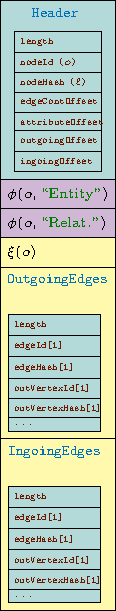
\includegraphics[height=.8\textheight]{/mnt/DEC4763AC47614CD/thesis/imgs/10nesting/test}
\caption{Extending the serialized graph data structure presented for graph join for the nesting operation. In particular, the present data structure extends each vertex representation in $VertexVals$ (Figure \vref{fig:graphstructure}) in order to fully supports the nested graph data model:
entities and relationships may now be contained into another data node (either a vertex or an edge). The first block of the serialized data structure contains the pointers towards the memory regions containing data which may vary in size. The fuchsia nodes remark the memory spaces where such data containments may be stored. Moreover, ingoing edges are stored as well as outgoing edges. }\label{nestedGraphVertex}
\end{figure}
\begin{algorithm}[!t]
	\caption{Two HOp Separated Patterns Algorithm (THoSP)}\label{alg:THoSPAlgorithm}
	\begin{adjustbox}{max width=\textwidth}
		\begin{minipage}{1.2\linewidth}
			\begin{algorithmic}[1]
				\Procedure{PartitionHashJoin}{$(g_V,\gamma_V),({g_E},\gamma_E^{src},\gamma_E^{dst}),\theta;\; \nested$}:
				\State \textsc{File} $AdjFile$ = \textsc{Open}($\nested$);
				\State \textsc{File} $Nesting$ = \textsc{Open}(\textbf{new});
				\State \textsc{Adjacency} $toSerialize$ = \textbf{new} \textsc{Map<Vertex,<Edge,Vertex>>}();
				\State {$\alpha:=g_V\cap {g_E}\backslash(\gamma_V\cup\gamma_E)$;}
				\For{\textbf{each vertex} $v$ in $AdjFile$}
				\If{$\alpha(v)$} \Comment{If $v$ matches the common subpattern $\alpha$. E.g., If $v$ is a \textsc{Paper}}
				\For {\textbf{each} $\gamma_V(u,e,v)$} \Comment{For each expansion of $v$ matching the pattern $\gamma_V$}
					\State{$u':=dt(1,dt(0,u))$} \Comment{Generate the id associated to the to-be nested vertex}
					\State{$NestingIndex$.write($\Braket{u',u}$)} \Comment{$\gamma_E^{src}. $Associated to $u'$ the elements matched by $\gamma_V$}
					\State{$NestingIndex$.write($\Braket{u',e}$)}
					\State{$NestingIndex$.write($\Braket{u',v}$)} \Comment{In our running example, only this element will be returned}
					\For {\textbf{each} $\gamma_V(w,e',v)$} 
						\If{$\gamma_E(v,e,u,e',w)$}
							\State{$w':=dt(1,dt(0,w))$} 
							\State{$\varepsilon:=dt(1,dt(u,w))$} \Comment{Generate the nested edge}
							\State{$NestingIndex$.write($\Braket{\varepsilon,u}$)} \Comment{$\gamma_E^{src}. $Associated to $u'$ the elements matched by $\gamma_V$}
							\State{$NestingIndex$.write($\Braket{\varepsilon,e}$)}
							\State{$NestingIndex$.write($\Braket{\varepsilon,w}$)}
							\State{$NestingIndex$.write($\Braket{\varepsilon,e'}$)}
							\State{$NestingIndex$.write($\Braket{\varepsilon,v}$)} \Comment{In our running example, only this element will be returned}
							\State{$toState$.put($u'$,$\Braket{\varepsilon,w'}$)}
						\EndIf
					\EndFor
				\EndFor
				\EndIf
				\EndFor
				$AdjFile$.serialize($toSerialize$);
				
				\EndProcedure
			\end{algorithmic}
	\end{minipage}
\end{adjustbox}
\end{algorithm}
\begin{table*}[!t]
	\centering
\begin{tabular}{@{}cr|rr@{}}
	\toprule
	{\textbf{Operands' Vertices}} & Matched Graphs  & {\textbf{General Nesting} (ms)} & {\textbf{THoSP} (ms)}  \\	
	\midrule
	$10$ & $3$ &  0.57       & 0.11\\
	$10^2$ & $58$  & 0.73        & 0.14\\
	$10^3$  & $968$  & 2.78   & 0.46\\
	$10^4$ & $8,683$   & 152.11   & 4.07\\
	$10^5$ & $88,885$   & 14,015.00 & 43.81 \\
	$10^6$  & $902,020$  &  1,579,190.00      & 563.02\\
	$10^7$ & $8,991,417$   &  $>$1H      & 8,202.93\\
	$10^8$ & $89,146,891$   &  $>$1H      & 91,834.20\\
	\bottomrule
\end{tabular}
	%\end{minipage}
	\caption{Comparing the performances of the THoSP algorithm with the naive General Nesting algorithm. This comparison shows that the previously defined algorithm has a worse performance than the THoSP one. }
	\label{tab:comparisonTwo}
\end{table*}


The main data structure over which this algorithm relies  is presented in Figure \vref{nestedGraphVertex}: it shows that minor changes have been applied to the original data structure that was used to serialize graph within the graph join scenario. %Moreover, in this case we mark with different hash values the vertices within the data structure satisfying different predicates within the predicates. 
Given that the data structure requires a simple linear visit of the graph, no additional primary and secondary data structures are required. Nevertheless, during our serialization phase we provide both a primary index for accessing external informations (\textit{VertexIndex}) and the serialization of all the vertices' adjacency lists, which is going to be used for traversing the graph (\textit{VertexVals}). In our straightforward implementation, hash values are here used only as placeholders for the nodes' labels used within the patterns but, given that vertices are not sorted by hash value as for graph joins, we keep the hash fields for both backward compatibility and in order to make graph joins possible for nested graphs, too.

Finally, Algorithm \vref{alg:THoSPAlgorithm} provides the desired implementation of the THoSP algorithm: we can observe that THoSP, contrariwise to the graph join operator, the data serialization is not included because no additional data and preprocessing steps are performed in order to provide a computational enhancement. The main memory is used to create the graph (represented as an adjacency list) that is going to be later on serialized using the same data structure used for providing the result for graph joins, that is an adjacency list where only the vertices' and edges' id appear. This choice is also done both for backward compatibility and for representing the nesting containment as a separate data structure. We can easily observe that this approach may slow down the whole algorithm, that can be quickened by directly storing the graph representation in secondary memory by using linear hashing. The nesting data structure is stored in a file as a set of pairs $\Braket{u,v}$, where $u$ represents the containing object and $v$ represents the content. By doing so, we omit the \texttt{Group By} cost which affects the previously seen query languages, thus allowing to an overall better performance. Even in this case, a join is performed between the two nested patterns: this is evident from the two nested for loops appearing in the algorithm. 

Table \ref{tab:comparisonTwo} provides a comparison between the general Nesting Algorithm and over the THoSP implementation of the query provided in our running example, under the assumptions that are going to be soon introduced in the next section. In particular, while THoSP increases linearly alongside the data size, the general nesting algorithm grows quadratically, thus quickly leading to a intractable time evaluation for big data scenarios. Hereby, the THoSP algorithm is going to be used in comparisons with other problem-specific queries on different query languages and data structures.